\begin{equation*}
% the lanes take the site's --mred (#7a2518); the link boxes are white-outlined, filled with the ink's complement
\definecolor{lanecolor}{RGB}{122,37,24}\colorlet{paper}{-.}%
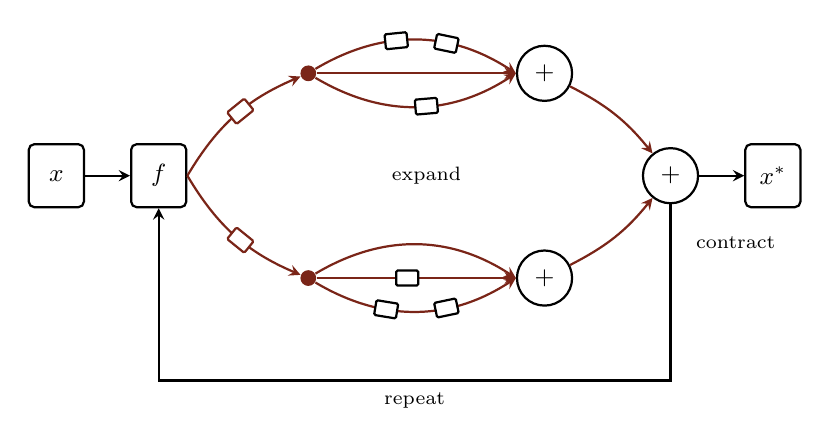
\begin{tikzpicture}[
  inst/.style={draw, rounded corners=2pt, thick, minimum width=7mm, minimum height=8mm, font=\small},
  fold/.style={draw, circle, thick, minimum size=7mm, font=\small},
  place/.style={circle, fill=lanecolor, minimum size=2mm, inner sep=0pt},
  hop/.style={thick, ->, >=stealth},
  lane/.style={thick, ->, >=stealth, color=lanecolor},
  link/.style={draw, fill=paper, thick, rounded corners=0.5pt, minimum width=2.8mm,
               minimum height=1.9mm, inner sep=0pt},
  note/.style={font=\scriptsize}
]
\node[inst] (x) at (0,0)   {$x$};
\node[inst] (f) at (1.3,0) {$f$};
\draw[hop] (x) -- (f);
% the root deals the frontier over its peers
\node[place] (p1) at (3.2,1.3)  {};
\node[place] (p2) at (3.2,-1.3) {};
\draw[lane] (f.east) to[bend left=18]  node[link, pos=0.55, sloped] {} (p1);
\draw[lane] (f.east) to[bend right=18] node[link, pos=0.55, sloped] {} (p2);
% each peer deals its part over its own peers and merges their answers
\node[fold] (m1) at (6.2,1.3)  {$+$};
\node[fold] (m2) at (6.2,-1.3) {$+$};
\foreach \ang in {-32,0,32} {
  \draw[lane] (p1) to[bend left=\ang] (m1.west);
  \draw[lane] (p2) to[bend left=\ang] (m2.west);
}
\path (p1) to[bend left=32]  node[link, pos=0.4, sloped] {} node[link, pos=0.65, sloped] {} (m1.west);
\path (p1) to[bend left=-32] node[link, pos=0.55, sloped] {} (m1.west);
\path (p2) to[bend left=0]   node[link, pos=0.45, sloped] {} (m2.west);
\path (p2) to[bend left=-32] node[link, pos=0.35, sloped] {} node[link, pos=0.65, sloped] {} (m2.west);
% the root merges the peers' answers: the superstep boundary
\node[fold] (m) at (7.8,0) {$+$};
\draw[lane] (m1) to[bend left=12]  (m);
\draw[lane] (m2) to[bend right=12] (m);
\node[inst] (xs) at (9.1,0) {$x^{*}$};
\draw[hop] (m) -- (xs);
% the back edge: the frontier one pass leaves is the next pass's
\draw[hop] (m.south) -- (7.8,-2.6) -- (1.3,-2.6) -- (f.south);
\node[note] at (4.7,0) {expand};
\node[note, anchor=west] at (8.0,-0.85) {contract};
\node[note] at (4.55,-2.85) {repeat};
\end{tikzpicture}
\end{equation*}
